% Time-stamp: <Thu 2022-02-03 14:58 svarrette>
% ==============================================================================
% cv-varrette-en.tex -- main LaTeX file of my personal CV
%
% Copyright (c) 2009-2011 Sebastien Varrette <Sebastien.Varrette@uni.lu>
% .             http://varrette.gforge.uni.lu
%
% .     ______     __          ____    __     __                  _   _
% .    / ___\ \   / /         / ___|   \ \   / /_ _ _ __ _ __ ___| |_| |_ ___
% .   | |    \ \ / /   _____  \___ \    \ \ / / _` | '__| '__/ _ \ __| __/ _ \
% .   | |___  \ V /   |_____|  ___) |    \ V / (_| | |  | | |  __/ |_| ||  __/
% .    \____|  \_/            |____(_)    \_/ \__,_|_|  |_|  \___|\__|\__\___|
%
% ==============================================================================
% This work is licensed under the CC-by-nc-sa 3.0 licence (see LICENCE file).
% For more details, visit:  http://creativecommons.org/licenses/by-nc-sa/3.0/
%
% For more info about this work, see the README file
% ==============================================================================
\documentclass{cv}

\usepackage{_style}


\begin{document}
% ---------- Header -----------
\begin{chapeau}
  \begin{adresse}
    {\Large\textbf{Sebastien VARRETTE, PhD}}\\
    \ligne\\
    \textbf{Research Scientist, Head Research Computing and HPC operations}\\
    \textbf{Management, Security and Performance of HPC systems}\\
    %\textbf{15 years of experience in Linux HPC systems}\\
    \ligne\\
    Phone: +33(0)6~74~57~90~05\\
    E-mail:    \url{Sebastien.Varrette@uni.lu}\\
    Home page: \url{http://varrette.gforge.uni.lu}\\
    GPG Key ID: \href{https://pgp.mit.edu/pks/lookup?op=vindex&search=0x5D08BCDD4F156AD7}{5D08BCDD4F156AD7}
  \end{adresse}
  \begin{etatcivil}
    %\includegraphics[width=0.2\textwidth]{Images/cv.jpg}
    \photo{Images/sv.jpg} %MyPhoto}

    Born on November 27th, 1979 (in France)\\
    Married (2004), two children (2007,2010)\\
  \end{etatcivil}
\end{chapeau}
% -----------------------------
\vspace*{0.5em}
\noindent\rule{\textwidth}{0.4pt}

\emph{Short bio:}
With more than 14 years of postdoctoral and team management experience, Dr. Varrette is Research Scientist within the University of Luxembourg.
Expert in the deployment and management of High Performance Computing (HPC) systems, he is leading the University’s HPC and Big Data platform, and the associated expert team managing and supporting this facility.\\
In parallel, he is pursuing his research in the domains of the security and performance of parallel and distributed computing platforms, such as HPC, Cloud Computing or Data Analytics infrastructures.
His research contributions led to more than 80 publications in high-level scientific journals, or international conference proceedings while co-authoring 4 books. He has a strong involvement in the community with reviewing roles in impact journals, conferences organization (e.g., IEEE CloudCom) and the participation to more than 50 conference program committee.\\
Finally, he takes part for the management committee and represents Luxembourg within multiple EU HPC projects, such as \href{http://www.prace-ri.eu/}{PRACE} (acting Advisor), \href{https://www.castiel-project.eu/}{CASTIEL}, \href{http://www.etp4hpc.eu/}{ETP4HPC} or several COST actions. He has also concrete contributions in several strategic projects linked to HPC developed with multiple key decision makers in the Luxembourg context, either from the private sector or at the governmental level (Ex: EuroHPC MeluXina Supercomputer). He's also acting as HPC expert for the European Commission in the Enhanced Regional EU-ASEAN Dialogue Instrument (E-READI) program.


%\iffullcv{
\noindent\rule{\textwidth}{0.4pt}

\vspace{1em}
\begin{tabular}{ll}
  \textsc{Technical / Management} & \acf{HPC}, \acf{BD} \& Cloud technologies.
  \\
  \textsc{Expertise:}& Managing large-scale \ac{HPC} and Data analytics systems since 2003
                       (Linux environment)
  \\
                                  & \textbf{HPC Team Leader since 2007} (Head, Uni.lu HPC facility)
                                  % \offset \offset \underline{\textit{Keywords:}} HPC, Debian, Xen, Puppet,
                                  % OpenLDAP, git\\
  \\
  \textsc{Main research domains}: & Security and Performance Evaluation of Distributed
                                    Computing Platforms \\ % (clusters, grids or clouds).\\
  \iffullcv{
                                  & \emph{Relevant contributions per domains}: \\
                                  % & Main achievements:\\
                                  & \offset HPC, Perf. \& Energy efficiency: \cvcite{DVB_SPECTS08,JVOB_EELSDS13,VGPBP_SBACPAD13,VPGBB_ICPP14,EVB_CLOUD16,OLADMFGGLLRMOPPPSSV_NESUS_COSTBook_Chap5,OV_NESUS_COSTBook_SubChap5,EVPB_TCC_19,VPKDB_PPAM19,MVPPB_CCGRID20,PVB_APF21,VKPKPCB_PEARC21} \\
                                  & \offset Security of Distributed Systems (incl. blockchains): \cite{BVP_CLOUD11,BVB_SiiS11,DRTV_FoundationCoding15,DRTV_ThCode18,IVP_ICOIN18,DLTV_Blockchains18,DLTV_Blockchains19,DLTV_Blockchains22,DLRTV_NFT22}\\
                                  & \offset Crash/cheating faults tolerance \cvcite{VRL_SBAC04,KRJV_EGC05, RV_Pasco07,Var_phD07,GGPV_PDP09,MVBSK_CAMWA12,MVB_CEC2013,MVJB_NSS14,MVB_Evostar2016}\\
                                  & \offset Code Obfuscation \cvcite{VTB_NIDISC13,BVB_NSS13}, Secure IaaS Cloud \cvcite{BVP_CLOUD11, BVB_Renpar11, BVB_TSI12} \\

                                  %& \offset  Design of the authentication system of Grid'5000
                                  % \cvcite{VGMRL_Gada05}\\
                                  %& \offset  Developing security awareness by education \cvcite{DRTV_ThCode07,BCCDV_DistSyst11_Chap11,DRTV_FoundationCoding15,DLTV_Blockchains18}
                                  % & \offset \offset \underline{\textit{Keywords:}} Grid Computing, Cloud, Security,
                                  % Fault-Tolerance, Authentication\\
                                  % \\
                                  % \multicolumn{2}{l}{I am a quick learner and a good communicator with the
                                  % ability to work within multi-cultural teams.}
  }
  \textsc{Books} \ifShortOrFull{\cite{VB_Prog_C07,DRTV_FoundationCoding15,DRTV_ThCode18,DLTV_Blockchains22,DLRTV_NFT22}}:
                                  &\\
                                  & \vspace*{-1em}
                                    \href{http://varrette.gforge.uni.lu/books/programmation-avancee-c/}{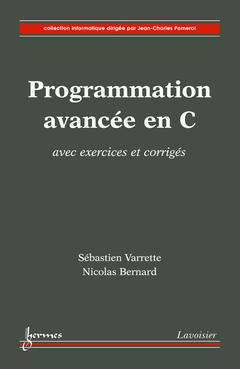
\includegraphics[height=8em]{cover-programmation-avancee-c.jpg}}
                                    \href{http://varrette.gforge.uni.lu/books/theorie-des-codes/}{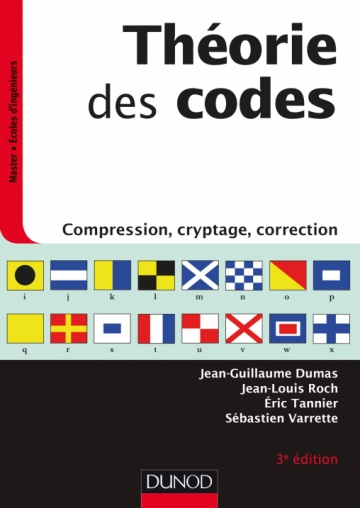
\includegraphics      [height=8em]{cover-theorie-des-codes.jpg}}
                                    \href{http://varrette.gforge.uni.lu/books/foundations-of-coding/}{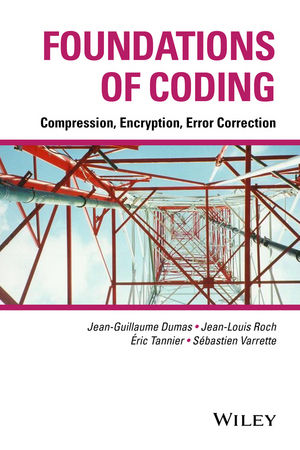
\includegraphics  [height=8em]{cover-foundations-of-coding.jpg}}
                                    \href{http://varrette.gforge.uni.lu/books/blockchains/}{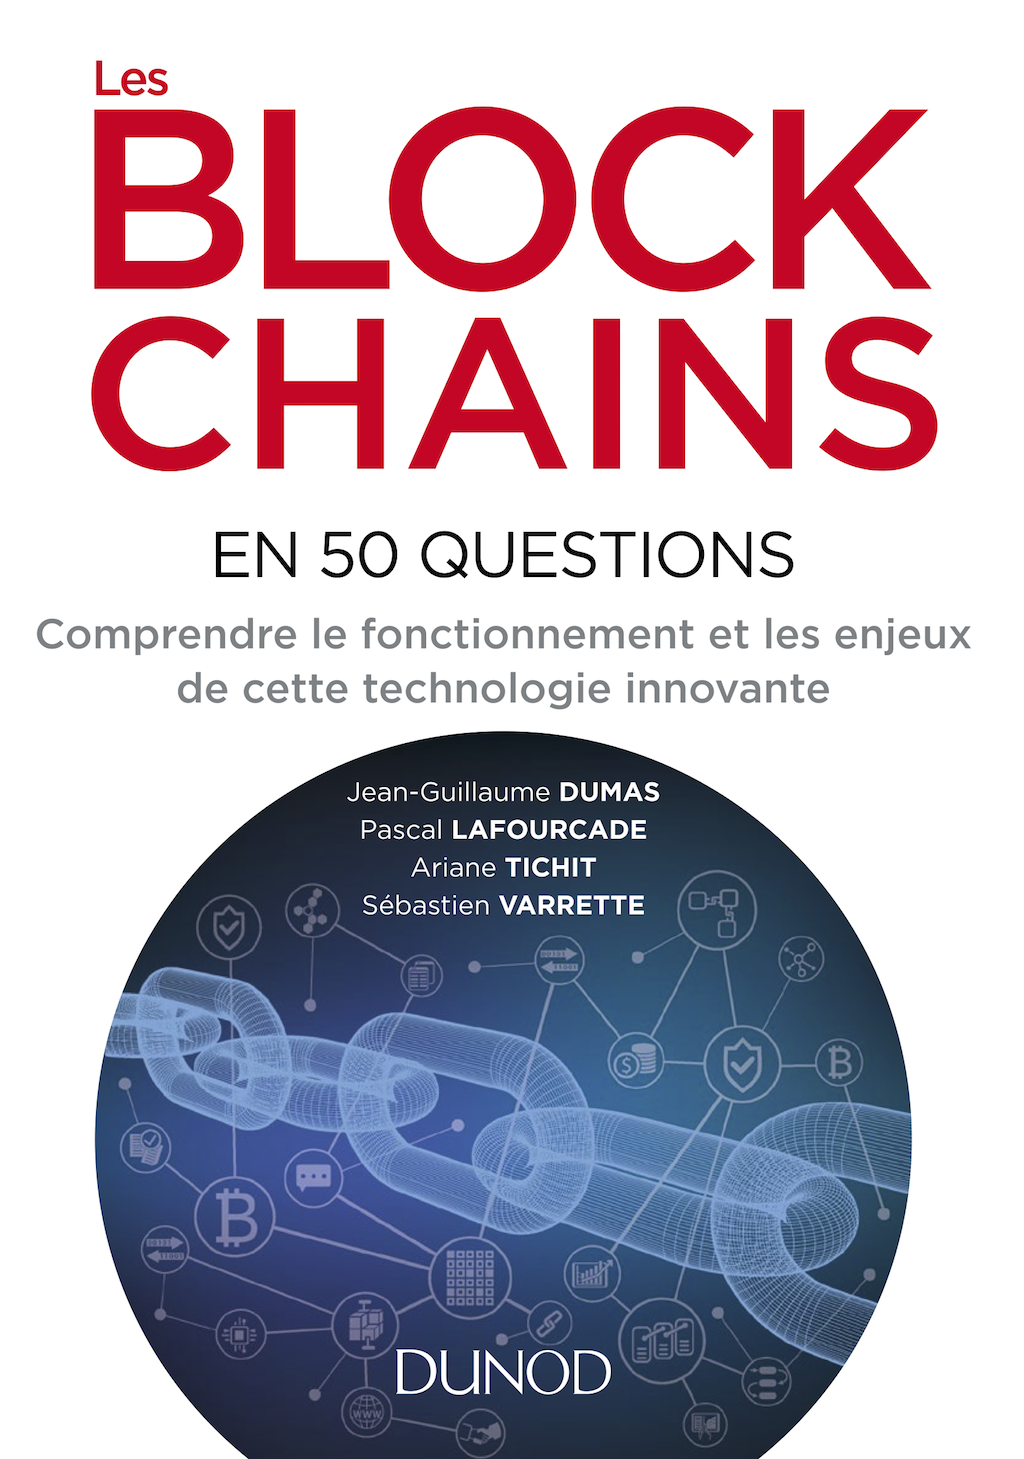
\includegraphics            [height=8em]{cover-blockchains.png}}
                                    \href{http://varrette.gforge.uni.lu/books/nft/}{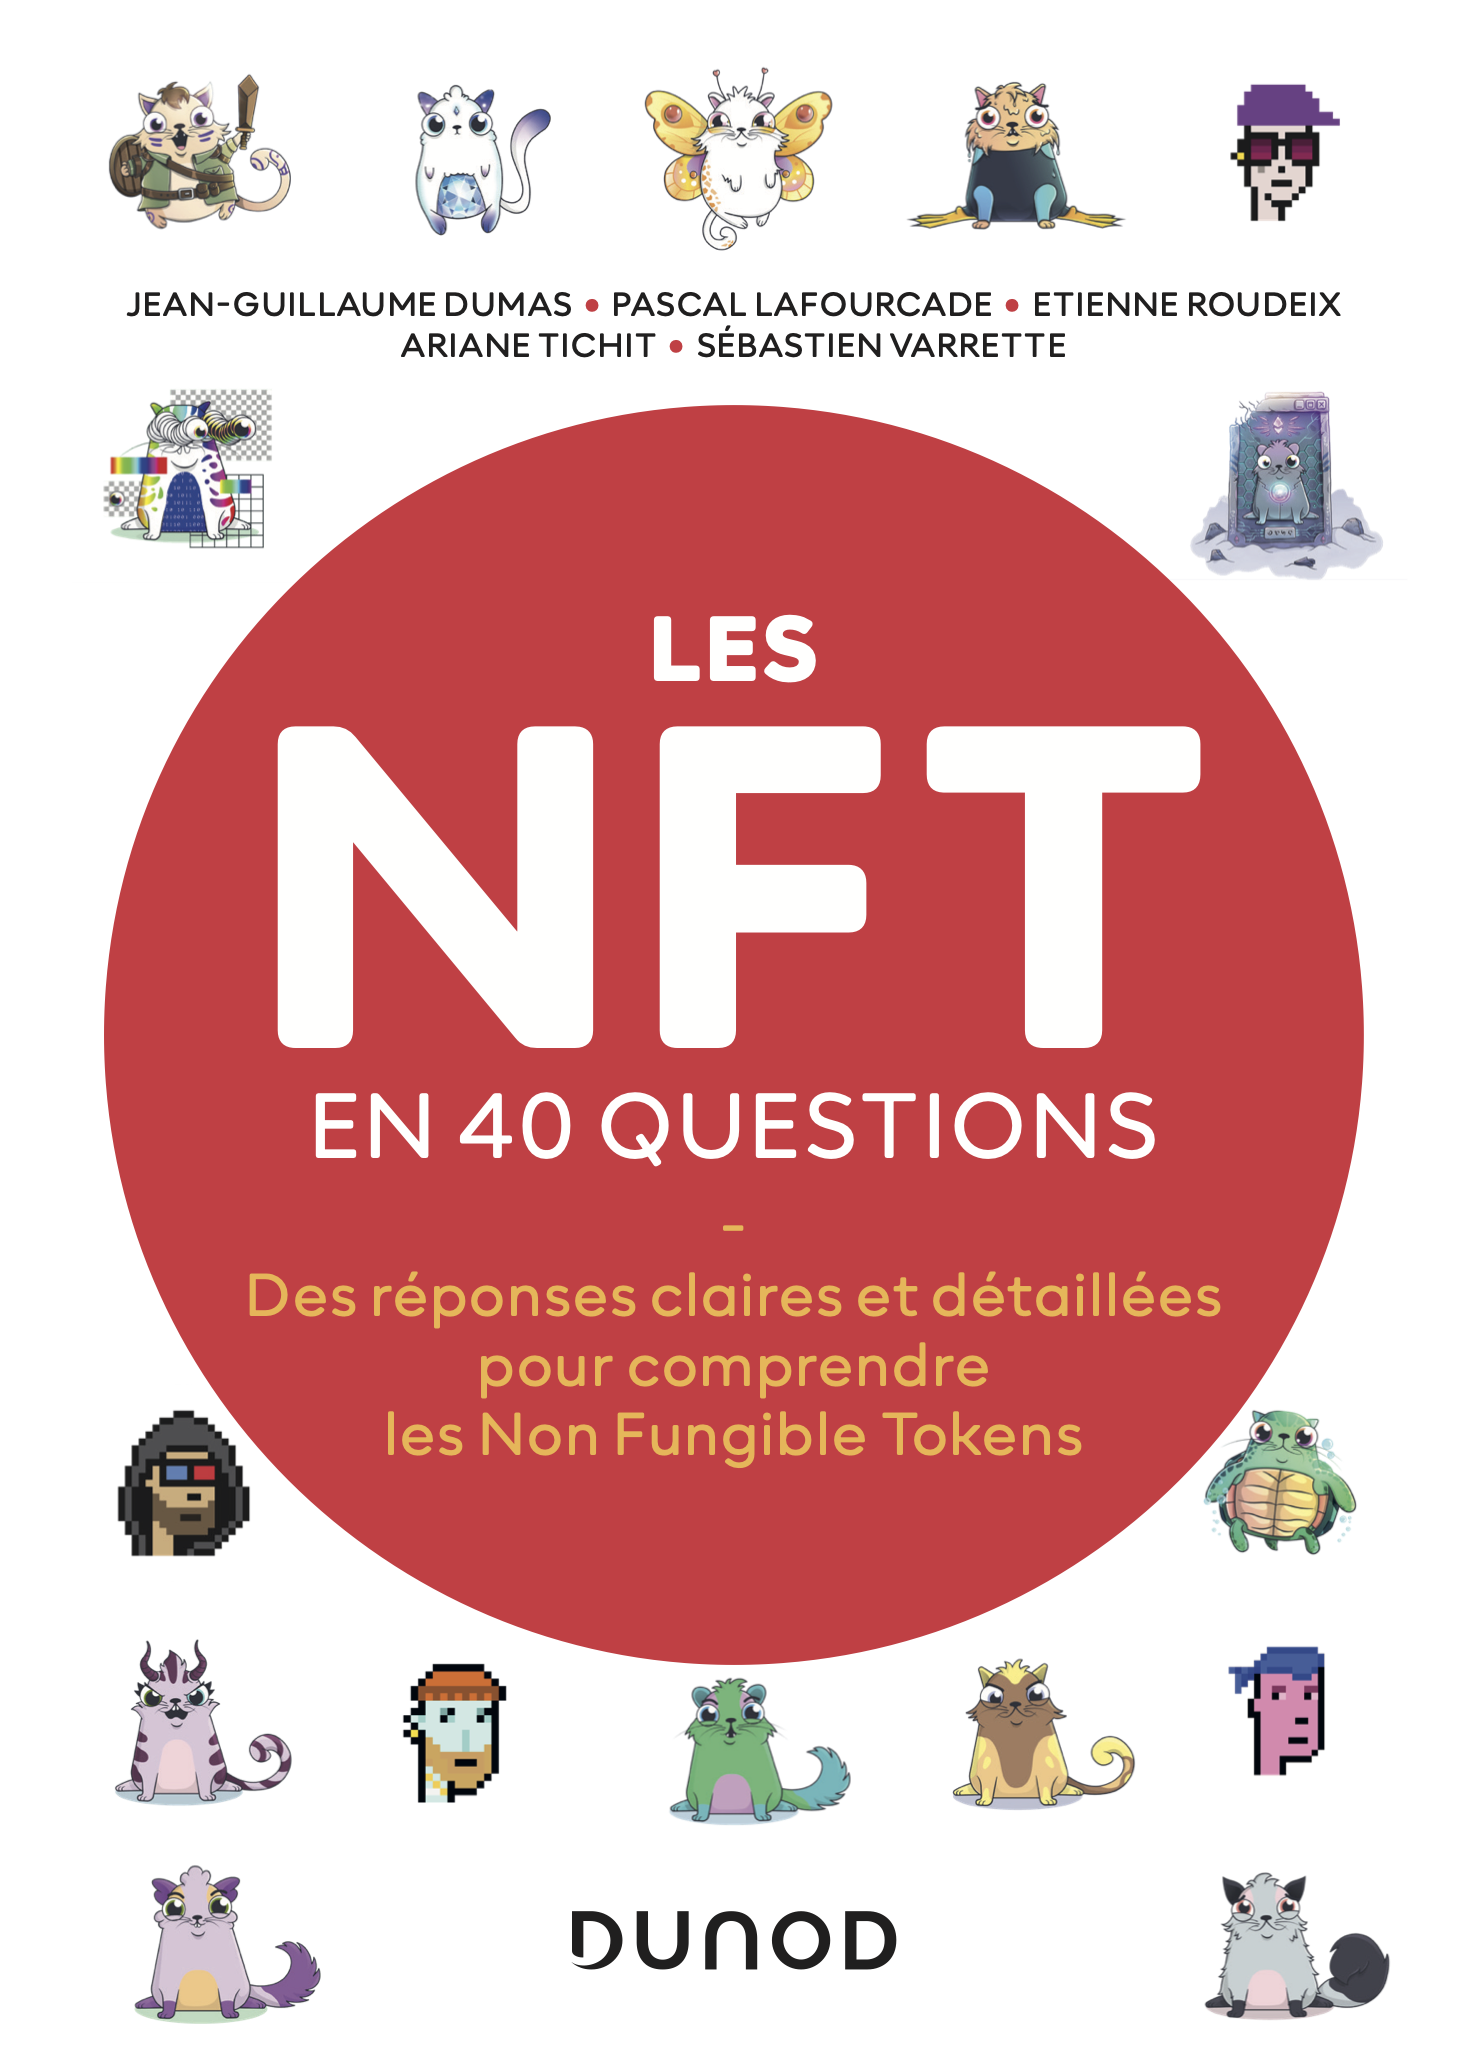
\includegraphics                    [height=8em]{cover-nft.png}}
  \\
\end{tabular}
\ifShortOrFull{\vspace{-1.5em}}
%}

% ---------- Education -----------
\ifShortOrFull{
  % Time-stamp: <Lun 2013-05-20 16:39 svarrette>
% ===============================================================================
% _education.tex -- my personal education
% 
% Copyright (c) 2009-2011 Sebastien Varrette <Sebastien.Varrette@uni.lu>
% .             http://varrette.gforge.uni.lu
%
% ==============================================================================
% This file is part of my CV (see 'cv-varrette-en.tex' and README)
%
% This work is licensed under the terms of the Creative Commons CC-by-nc-sa 3.0
% licence (see LICENCE). For more details, visit:
% .         http://creativecommons.org/licenses/by-nc-sa/3.0/
% ==============================================================================

\begin{rubriquetableau}[\offsetintab]{Education}
    2007
    & \textsc{Ph.D. in Computer Science},
    \hfill with honours  (\textsl{Excellent/Outstanding})\\
    & \vspace{-0.8em}\acf{UL} \& \acf{INPG}\\
    \ifnum\pdfstrcmp{\cvtype}{\cvtiny}=0
    \else
    & \offset Thesis: \emph{Security in Large Scale Distributed Systems:
      Authentication and Result Checking}\\
    & \offset Advisors\,: Franck Lepr�vost (\ac{UL}) \& Jean-Louis Roch (\ac{INPG})\\
    \\
    \fi
    2003
    & \textsc{M.Sc. in Computer Science} \hfill with honours (\textsl{TB/First Class})\\
    & Speciality: Cryptology, Security and Information Coding (CSCI), \hfill rank: 1st\\
    \ifnum\pdfstrcmp{\cvtype}{\cvtiny}=0
    \else
    & \acf{INPG} \& \acf{UJF}\\
    % & \offset Thesis: \emph{Securing Peer-to-Peer Computing in Grid Environments}\\
    % & \offset Advisor: Jean-Louis Roch (\ac{INPG}) \\
    \fi
    2003
    & \textsc{Master's Degree in Engineering}
    (\TelecomsENSIMAG)\hfill with honours (\textsl{B/2.1})\\
    & Speciality: Computer Sciences and Telecommunications \hfill rank: top 10\%\\
   \\
    \ifnum\pdfstrcmp{\cvtype}{\cvtiny}=0
    \else
    1997 -- 2000
    & \textsc{Advanced Mathematics and Physics studies} \\
    & \offset For the competitive entrance to the French engineering schools
    \\
    1997
    & \textsc{Scientific "Baccalaur�at"} (French "A" levels) \hfill with honours (\textsl{B/2.1})
    \fi
\end{rubriquetableau}


% ===============================================================================
% eof
% 
% Local Variables:
% mode: latex
% mode: flyspell
% mode: auto-fill
% fill-column: 80
% End:
 % ALL
}

% ---------- Employment -----------
\iffullcv{%\ifShortOrFull{
  \vspace*{-1.5em}
  % Time-stamp: <Wed 2019-04-10 18:00 svarrette>
% ==============================================================================
% _employment.tex -- Details of my employments
%
% Copyright (c) 2009-2011 Sebastien Varrette <Sebastien.Varrette@uni.lu>
% .             http://varrette.gforge.uni.lu
%
% ==============================================================================
% This file is part of my CV (see 'cv-varrette-en.tex' and README)
%
% This work is licensed under the terms of the Creative Commons CC-by-nc-sa 3.0
% licence (see LICENCE). For more details, visit:
% .         http://creativecommons.org/licenses/by-nc-sa/3.0/
% ==============================================================================

\begin{rubriquetableau}[\offsetintab]{Employment}
    2007 -- now  & \textsc{Research Scientist} (\UL, Luxembourg)\\
    2004 -- 2007 & \textsc{Research Assistant} (\UL, Luxembourg)\\
    2003         & \textsc{IT (Lab) and HPC System Manager} (\ID, Grenoble, France),
\end{rubriquetableau}

% ==============================================================================
% eof
%
% Local Variables:
% mode: latex
% mode: flyspell
% fill-column: 80
% End:

}

% ---------- Awards -----------
\ifShortOrFull{
  \vspace*{-0.5em}
  % Time-stamp: <Mon 2018-08-20 22:21 svarrette>
% ==============================================================================
% _awards.tex --
%
% Copyright (c) 2018 Sebastien Varrette <Sebastien.Varrette@uni.lu>
% .             http://varrette.gforge.uni.lu
%
% ==============================================================================
% This file is part of my CV (see 'cv-varrette-en.tex' and README)
%
% This work is licensed under the terms of the Creative Commons CC-by-nc-sa 3.0
% licence (see LICENCE). For more details, visit:
% .         http://creativecommons.org/licenses/by-nc-sa/3.0/
% ==============================================================================

\begin{rubriquetableau}[\offsetintab]{Awards}
  2018  & \textsc{IEEE ICoin 2018}: Best Paper Award       \hfill\cvcite{IVP_ICOIN18}\\
  2014  & \textsc{IEEE NSS 2014}: Best Student Paper Award \hfill\cvcite{MVJB_NSS14}\\
\end{rubriquetableau}

% ==============================================================================
% eof
%
% Local Variables:
% mode: latex
% mode: flyspell
% fill-column: 80
% End:

}
\unlesstinycv{
  \iffullcv{\clearpage}
  % ---------- Teaching-----------
  \ifShortOrFull{
    % Time-stamp: <Wed 2011-02-23 14:56 svarrette>
% ==============================================================================
% _teaching.tex -- details of the lectures carried out
% 
% Copyright (c) 2009-2011 Sebastien Varrette <Sebastien.Varrette@uni.lu>
% .             http://varrette.gforge.uni.lu
%
% ==============================================================================
% This file is part of my CV (see 'cv-varrette-en.tex' and README)
%
% This work is licensed under the terms of the Creative Commons CC-by-nc-sa 3.0
% licence (see LICENCE). For more details, visit:
% .         http://creativecommons.org/licenses/by-nc-sa/3.0/
% ==============================================================================

\begin{rubriquetableau}[\offsetintab]{Teaching Experience}
    2008 -- now  & \textsc{Parallel \& Grid Computing}, \textsc{Middleware}
    \hfill Master MICS2 (UL)\\
%    \\
    2004 -- 2007 & \textsc{Programming Techniques I}   \hfill Bachelor I1/CUT1 (UL)\\
    & \textsc{Advanced Programming in C, C++ and Java} \hfill Bachelor I2 (UL)\\
    & \textsc{System Administration and Network Security} \hfill Master CSCI2 (UJF)\\
%    \\
    2006         & \textsc{Cryptology and Network Security}\\
    & \offset Master in Computer Science
    (\href{http://www.uy1.uninet.cm/}{Univ. of Yaound� I}, Cameroon)
\end{rubriquetableau}

% ==============================================================================
% eof
% 
% Local Variables:
% fill-column: 80
% mode: latex
% mode: flyspell
% mode: auto-fill
% End:

  }

  % ---------- Additional information ----------
  \iffullcv{
    % Time-stamp: <Wed 2011-06-08 11:19 svarrette>
% ===============================================================================
% _other.tex -- other information
% 
% Copyright (c) 2009-2011 Sebastien Varrette <Sebastien.Varrette@uni.lu>
% .             http://varrette.gforge.uni.lu
%
% ==============================================================================
% This file is part of my CV (see 'cv-varrette-en.tex' and README)
%
% This work is licensed under the terms of the Creative Commons CC-by-nc-sa 3.0
% licence (see LICENCE). For more details, visit:
% .         http://creativecommons.org/licenses/by-nc-sa/3.0/
% ==============================================================================

\begin{rubriquetableau}[\offsetintab]{Additional Information}
    % & Driver's Licence\\
    \textbf{Languages}
    & \textsc{French} (native language), \textsc{English}
    (fluent) and \textsc{German} (basic knowledge)
    \\
    \textbf{Sports}
    & Karate (Black belt -- {\small 2nd DAN}, \acf{DIF}), Jogging, Badminton, Ski
    etc.
    \\
    \textbf{Hobbies}
    & Collectible Card Games (VTES), Video Games etc.\\
\end{rubriquetableau}

% ===============================================================================
% eof
% 
% Local Variables:
% mode: latex
% mode: flyspell
% mode: auto-fill
% fill-column: 80
% End:

  }
  %\ifshortcv{\clearpage}
  %\ifshortcv{% Time-stamp: <Wed 2018-08-29 14:05 svarrette>
% ===============================================================================
% _phd_board.tex -- Participation to PhD boards
%
% Copyright (c) 2009-2018 Sebastien Varrette <Sebastien.Varrette@uni.lu>
% .             http://varrette.gforge.uni.lu
%
% ==============================================================================
% This file is part of my CV (see 'cv-varrette-en.tex' and README)
%
% This work is licensed under the terms of the Creative Commons CC-by-nc-sa 3.0
% licence (see LICENCE). For more details, visit:
% .         http://creativecommons.org/licenses/by-nc-sa/3.0/
% ==============================================================================

\begin{rubriquetableau}[\offsetintab]{Participation to Ph.D Boards}
  Oct. 2016 & \textsc{Alban Rousset}, Institut FEMTO-ST, Université de Franche-Comté.
 \emph{Contribution à la distribution et à la synchronisation des Systèmes Multi-Agents sur les super-calculateurs}, Examinateur
  \\
  Sept. 2018 & \textsc{Gabriele Pozzetti}, University of Luxembourg\\
  & \emph{A dual-grid  multiscale  approach  to CFD-DEM couplings  for multiphase flow}, Jury member
  \\
  Dec. 2018 & \textsc{David Guyon}, University of Rennes I\\
  & \emph{Energy-efficient Cloud Elasticity for Data-driven Applications} (pending exact title), Jury Member
  \\
\end{rubriquetableau}


% ===============================================================================
% eof
%
% Local Variables:
% mode: latex
% mode: flyspell
% mode: visual-line
% fill-column: 80
% End:
}

  % ---------- Graduate student supervision -----------
  % Time-stamp: <Lun 2015-03-16 23:10 svarrette>
% ===============================================================================
% _supervision.tex -- Students I used to supervise
% 
% Copyright (c) 2009-2011 Sebastien Varrette <Sebastien.Varrette@uni.lu>
% .             http://varrette.gforge.uni.lu
%
% ==============================================================================
% This file is part of my CV (see 'cv-varrette-en.tex' and README)
%
% This work is licensed under the terms of the Creative Commons CC-by-nc-sa 3.0
% licence (see LICENCE). For more details, visit:
% .         http://creativecommons.org/licenses/by-nc-sa/3.0/
% ==============================================================================

\begin{rubriquetableau}[\offsetintab]{Graduate Students Supervision}
    \textbf{PhD.}
    & \supervision{Jakub Muszy\'nski}{2011 -- 2015}{Cheating-Tolerance of Parallel and Distributed Evolutionary Algorithms in Desktop Grids and Volunteer Computing Systems}
    \\
    & \supervision{Beno\^it Bertholon}{2010 -- 2013}{CertiCloud \& JShadObf:
      Toward Integrity and Software Protection in Cloud Computing Platforms}
    \\
    \\
    \textbf{Master}
    & \supervision{Maxime Schmitt}{2014--2015}{RESIF and OpenStack Deployment}
    \\
    & \supervision{Ludovic Schoepps}{2014}{Design a REST API service to Monitor UL HPC Resources}
    \\
    & \supervision{Anna Giannakou}{2013}{Energy Efficiency in HPC environments}
    \\
    & \supervision{Valentin Plugaru}{2012 --}{Energy Efficiency of Hypervisors
      and Cloud middleware}
    \\
    & \supervision{S\'ebastien Martinez}{2012}{Source Code Obfuscation by mean
      of Evolutionary Algorithms}
    \\
    & \supervision{Fotis Georgatos}{2012 -- 2014} {System administrator of the
      \href{http://hpc.uni.lu}{UL HPC facility}}
    \\
    & \supervision{Mateusz Guzek}{2011}{System administration of cluster-based HPC systems}
    \\
    & \supervision{Beno�t Bertholon}{2009}{Integrity issues in distributed executions}
    \\
    & \supervision{Christophe Weis}{2009}{Optimizing hash functions and S-Box by GEP}
    \\
    & \supervision{Dominic Dunlop}{2008 -- 2009}{Using GAs to tune benchmarks for HPCs}
    \\
    & \supervision{Romain Cavagna}{2007 -- 2008}{Deployment of a GForge platform}
    \\
    \\
    \textbf{Bachelor}
    & \supervision{Hyacinthe Cartiaux}{2011 -- } {System administrator of the
      \href{http://hpc.uni.lu}{UL HPC facility}}
    \\
    & \supervision{Bernard Reichert}{2008}{Collision detection implementation  using CUDA}
\end{rubriquetableau}

% ===============================================================================
% eof
% 
% Local Variables:
% mode: latex
% mode: flyspell
% mode: auto-fill
% fill-column: 80
% End:

  \vspace{-0.5em}
  \iffullcv{\clearpage}
  % ---------- Participation PhD. Board -----------
  \iffullcv{% Time-stamp: <Wed 2018-08-29 14:05 svarrette>
% ===============================================================================
% _phd_board.tex -- Participation to PhD boards
%
% Copyright (c) 2009-2018 Sebastien Varrette <Sebastien.Varrette@uni.lu>
% .             http://varrette.gforge.uni.lu
%
% ==============================================================================
% This file is part of my CV (see 'cv-varrette-en.tex' and README)
%
% This work is licensed under the terms of the Creative Commons CC-by-nc-sa 3.0
% licence (see LICENCE). For more details, visit:
% .         http://creativecommons.org/licenses/by-nc-sa/3.0/
% ==============================================================================

\begin{rubriquetableau}[\offsetintab]{Participation to Ph.D Boards}
  Oct. 2016 & \textsc{Alban Rousset}, Institut FEMTO-ST, Université de Franche-Comté.
 \emph{Contribution à la distribution et à la synchronisation des Systèmes Multi-Agents sur les super-calculateurs}, Examinateur
  \\
  Sept. 2018 & \textsc{Gabriele Pozzetti}, University of Luxembourg\\
  & \emph{A dual-grid  multiscale  approach  to CFD-DEM couplings  for multiphase flow}, Jury member
  \\
  Dec. 2018 & \textsc{David Guyon}, University of Rennes I\\
  & \emph{Energy-efficient Cloud Elasticity for Data-driven Applications} (pending exact title), Jury Member
  \\
\end{rubriquetableau}


% ===============================================================================
% eof
%
% Local Variables:
% mode: latex
% mode: flyspell
% mode: visual-line
% fill-column: 80
% End:
}

  %\ifsmallcv{\clearpage}

  % ---------- Research Project ------------
  %\iffullcv{\clearpage}
  % Time-stamp: <Mar 2014-03-25 21:36 svarrette>
% ===============================================================================
% _research_project.tex -- Research projects I'm involved in (at various degrees)
% 
% Copyright (c) 2009-2011 Sebastien Varrette <Sebastien.Varrette@uni.lu>
% .             http://varrette.gforge.uni.lu
% 
% ==============================================================================
% This file is part of my CV (see 'cv-varrette-en.tex' and README)
% 
% This work is licensed under the terms of the Creative Commons CC-by-nc-sa 3.0
% licence (see LICENCE). For more details, visit:
% .         http://creativecommons.org/licenses/by-nc-sa/3.0/
% ==============================================================================

\begin{rubriquetableau}[\offsetintab]{Research Projects}
    2007 -- now  & \href{http://hpc.uni.lu}{UL HPC} (UL cumulative
    contribution: \textbf{5.7 M\euro{}}) \\
    2014 -- now & EU \href{http://www.cost.eu/domains_actions/ict/Actions/IC1305/}{\textsc{COST Action IC1305}}:
    {\small Network for Sustainable Ultrascale Computing (NESUS)}
    \\
    2011 -- 2013 & UL \textsc{EvoPerf} (UL contribution: 373 k\euro{})
    \\
    2010 -- 2012 &
    FNR CORE \href{http://greenit.gforge.uni.lu/}{\textsc{GreenIT}}
    (Total: 1,5 M\euro{}, FNR contribution: 432 k\euro{})
    % {\small holistic autonomic energy-efficient solution to manage, provision, and
    %   administer CC/HPC data centers} % WP7
    \\
    2010 -- 2012 & AFR PhD \textsc{Bertholon}
    (PHD-09-142; Scientific Advisor; Total/AFR contribution:
    110 k\euro{})\\
    & \offset
    {\small Confidentiality and Integrity Issues over Cloud Computing Platforms}
    \\
    2009 -- 2013 & EU \href{http://www.cost804.org/}{\textsc{COST Action IC0804}}:
    {\small Energy efficiency in large scale distributed systems}
    \\
    2009 -- 2013 &
    EU \href{http://www.coregrid.net/}{\textsc{CoreGrid}}
    % {\small Foundations, Software Infrastructures and Applications for large
    %   scale distributed, Grid and P2P Technologies (Trust and Security project)}
    \\
   2006 -- 2008 &
    ANR \href{http://www-lipn.univ-paris13.fr/safescale/}{\textsc{SafeScale-BGPR}}
    (ANR-05-SSIA-0005; ANR contribution: 68 k\euro{})
    % {\small Security \& Fault-tolerance to Exploit Safety ambient Computing in lArge
    %   scaLe Environments}
    \\
    2005 -- now & \href{http://www.grid5000.org}{\textsc{Grid'5000}} (technical committee)
    % {\small highly reconfigurable, controlable and monitorable experimental
    %   grid}
    \\
    2005 -- 2007 & FNR-SECOM \textsc{TeseGrad} (FNR contribution: 300 k\euro{})
    %{\small Techniques for Securing Grids and Ad-Hoc networks project}
    \\
    2004 -- 2007 &
    \href{http://www-fourier.ujf-grenoble.fr/~gillard/cryptalpes.html}{\textsc{CryptAlpes}}
    % {\small mathematical aspects of cryptography; security aspects of
    %   distributed/P2P computations}
    \\
    2004 -- 2006 & %Regional % PTP % Projet Thematique Prioritaire 
    \href{http://infographie.univ-lyon2.fr/~miguet/ragtime}{\textsc{RagTime}}
    (Total: 545 k\euro{}, Rh\^one-Alpes Region contribution: 217 k\euro{})
    % {\small Rh\^one-Alpes : Grille pour le Traitement d'Informations M�dicales
    %   (WP3: Acc\`es aux Donn\'ees et S\'ecurit\'e)}
    \\
\end{rubriquetableau}

% ===============================================================================
% eof
% 
% Local Variables:
% mode: latex
% mode: flyspell
% mode: auto-fill
% fill-column: 80
% End:


  % ---------- Professional development ----------
  \ifShortOrFull{
    % Time-stamp: <Mar 2014-03-25 21:29 svarrette>
% ===============================================================================
% _professional_dev.tex -- professionnal development
% 
% Copyright (c) 2009-2011 Sebastien Varrette <Sebastien.Varrette@uni.lu>
% .             http://varrette.gforge.uni.lu
% 
% ==============================================================================
% This file is part of my CV (see 'cv-varrette-en.tex' and README)
% 
% This work is licensed under the terms of the Creative Commons CC-by-nc-sa 3.0
% licence (see LICENCE). For more details, visit:
% .         http://creativecommons.org/licenses/by-nc-sa/3.0/
% ==============================================================================

\begin{rubriquetableau}[\offsetintab]{Professional Development}
    & IEEE Computer and Computational Intelligence society member\\
    & Organizer of various conferences\\
    & "\emph{Autorisation \`a Diriger des Recherches}" (ADR) granted on July, 2015\\ 
    &\\
    2009 -- now  & \textsc{Technical advisor} for
    \href{http://lcsb.uni.lu}{LCSB} and the
    \href{http://www.eco.public.lu/}{MECO} Ministry on HPC projects\\
    2007 -- now  & \textsc{\href{http://hpc.uni.lu}{UL HPC} Manager}.\\
    & \textbf{Cumulative Project Investment: 6.3 M\euro{}} {\small (as of 2015)}.\\
    & \offset \offset 400 computing nodes, 4284 cores, $R_{\text{peak}} =  49.92$ TFlops\\
    & \offset \offset 150 servers (74,6\% are Xen VMs)\\
    & \offset \offset NFS, GPFS, Lustre Storage (Total capacity: 4268 TB)\\
    & \offset \offset Management of a team of 4 system administrators\\
    & \\
    2007 -- now  & Manager of various IT services
    (\href{http://gforge.uni.lu}{Gforge @ Uni.lu}, Jabber etc.)\\ 
    2006         & \href{http://www.egide.asso.fr/}{EGIDE} mission for 3 weeks
    in Cameroon (master lecture -- Univ. of Yaoud� I)\\
    2005 & \textsc{Editorial Committee} for the definition of new \UL master and
    bachelor degrees % :\\
    % & \offset \offset Master of Science \emph{Security and Trust} and \emph{Security management} \\
    % & \offset \offset Bachelor \emph{Informatique de Gestion}
    \\
    2005 -- 2006 & \textsc{Editorial Committee}, \UL website (CMS selection \& management)\\
    2005 -- 2006 & \textsc{Faculty Council}, elected member (assistant representative)\\
    2000 -- 2002 & \textsc{Ensimag Junior Enterprise}, developer member\\
\end{rubriquetableau}


% ===============================================================================
% eof
% 
% Local Variables:
% mode: latex
% mode: flyspell
% mode: auto-fill
% fill-column: 80
% End:

    \ifshortcv{\clearpage}
  }

  % ---------- Participation -----------
  % % Time-stamp: <Mon 2011-06-06 17:39 svarrette>
% ===============================================================================
% _participation.tex -- Participa
% 
% Copyright (c) 2009-2011 Sebastien Varrette <Sebastien.Varrette@uni.lu>
% .             http://varrette.gforge.uni.lu
% 
% ==============================================================================
% This file is part of my CV (see 'cv-varrette-en.tex' and README)
% 
% This work is licensed under the terms of the Creative Commons CC-by-nc-sa 3.0
% licence (see LICENCE). For more details, visit:
% .         http://creativecommons.org/licenses/by-nc-sa/3.0/
% ==============================================================================

\begin{rubriquetableau}[\offsetintab]{Participation to PhD supervision}
    2011 -- 2013 & Scientific Advisor of the thesis of Jakub Muszy\'nski, \UL.
    Subject: \emph{Integrity aspects on grid and cloud platforms}
    \\
    
\end{rubriquetableau}


% \begin{rubriquetableau}[\offsetintab]{Affiliations / Memberships}
%     \textbf{Affiliations} & Computer Science and Communications (CSC) Research Unit
%     \hfill 2007 -- now \\
%     & Laboratory of Algorithmics, Cryptology and Security (LACS)
%     \hfill 2004 -- 2007\\
%     & Laboratoire Informatique et Distribution (ID-IMAG) \hfill 2003 -- 2007

%     \\
%     \textbf{Research}
%     & \textsc{Grid5000} / \textsc{Aladdin-G5K} (2004 -- now) \hfill
%     \miniurl{http://www.grid5000.org}\\
%     \textbf{projects}

%     & \textsc{Safescale} (2006 -- 2008):
%     Security And Fault-tolerance to Exploit Safety ambient Computing in lArge
%     scaLe Environments \hfill
%     \miniurl{http://www-lipn.univ-paris13.fr/safescale/} \\
%     & \textsc{Ragtime} (2004 -- 2006): Rh\^one-Alpes : Grille pour le Traitement
%     d'Informations M�dicales \hfill
%     \miniurl{http://liris.univ-lyon2.fr/~miguet/ragtime/}

%     \\
%     \textbf{Working}
%     & \textsc{Manager} of the HPC facilities @ UL\hfill 2007 -- now\\
%     \textbf{groups}
%     & \textsc{Technical Committee} in Grid5000, member \hfill 2005 -- now\\

%     &  \textsc{Program elaboration} for new degrees at
%     UL \hfill 2005 \\
%     & \offset $\bullet$  Master of Science \emph{Security and
%     Trust} and \emph{Security management} \\
%     & \offset $\bullet$ Bachelor \emph{Informatique de Gestion}\\

%     & \textsc{Editorial Committee} for the university web site \hfill 2005

%     \\
%     \textbf{Reviews} & International Journal of Parallel Programming (2006) and
%     various conferences

%     \\
%     \textbf{Events}
%     & \textsc{Program Committee}: \emph{Workshop on Desktop Grids and Volunteer
%     Computing Systems (PCGrid)}, part of  ACM CCGrid\hfill 2010 -- now\\
%     & \textsc{General Co-Chair}: 1st Luxembourg-Polish Workshop on Security and
%     Trust (LPWST'2010),
%     \emph{Workshop on Optimization Issues in Grid and Parallel Computing
%     Environments (OPTIM)}, part of IEEE HPCS\\

%     & \textsc{Co-funder}: \emph{Les Midis de la Science}, scientific lectures for
%     PhD students \hfill 2005
% \end{rubriquetableau}


% ===============================================================================
% eof
% 
% Local Variables:
% fill-column: 80
% mode: latex
% mode: flyspell
% End:

}
\iffullcv{\clearpage}
% ---------- Publications ----------
% ==============================================================================
% _publis.tex -- List of my personal publication
% 
% Copyright (c) 2009-2011 Sebastien Varrette <Sebastien.Varrette@uni.lu>
% .             http://varrette.gforge.uni.lu
% 
% This file is part of my CV (see 'cv-varrette-en.tex')
% 
% This work is licensed under the Creative Commons
% Attribution-NonCommercial-ShareAlike 3.0 Unported License (see LICENCE file)
% ==============================================================================
% 
% Based on the files produced by 'scripts/split_bibtex_per_type.pl'
% 

\def\bibfile{biblio-varrette}

\begin{rubrique}{Publications}

    {\small
      % search "varrette" in the domain "Engineering, Computer Science, Mathematics"
      \href{http://www.harzing.com/pop.htm}{Publish or Perish}: [
      Papers:29 | Citations:86 | Years:8 | h-index:6 | g-index:8 |
      hc-index:5,hI-index:1.80,hI-norm:4 |
      AWCR:12.40 | AW-index:3.52 | AWCRpA:4.93 | e-index:4.90 |
      hm-index:3.83,"22/02/2011" ] \\
   }
    
    % Summary of the publications
    \IfFileExists{__sub_\bibfile_summary.tex}{
      \input{__sub_\bibfile_summary}
    }{}


    \IfFileExists{__sub_\bibfile_main.tex}{
      \input{__sub_\bibfile_main}
    }{}
    
\end{rubrique}





% ==============================================================================
% eof
% 
% Local Variables:
% mode: latex
% mode: flyspell
% mode: auto-fill
% fill-column: 80
% End:



% ===========  Acronyms ===========
\begin{acronym}
  \acro{BD}{Big Data}
  \acro{CC}{Cloud Computing}
  \acro{CSC}[\href{http://csc.uni.lu}{CSC}]{Computer Science and Communications}
  \acro{DIF}[\href{http://www.ffkama.fr/direction-technique/formation/formationsfederales.php}{DIF}]{Federal Instructor Diploma}
  \acro{EA}{Evolutionary Algorithm}
  \acro{ETP4HPC}{European Technology Platform (ETP) in the area of HPC}
  % \acro{ENSIMAG}[\href{http://ensimag.grenoble-inp.fr/}{ENSIMAG}]{}
  \acro{HPC} {High Performance Computing}
  \acro{INPG}[\href{http://www.grenoble-inp.fr/}{INPG}]{Institut National Polytechnique de Grenoble}
  \acro{IaaS}{Infrastructure-as-a-Service}
  \acro{ID}[\href{http://www-id.imag.fr}{ID-IMAG}]{Laboratoire Informatique et Distribution}
  \acro{LACS}[\href{http://lacs.uni.lu}{LACS}]{Laboratory of Algorithmics, Cryptology and Security}
  \acro{NESUS}{Network for Sustainable Ultrascale Computing}
  \acro{NVAITC}{NVidia Artificial Intelligence (AI) Tech. Center}
  \acro{PRACE}[\href{http://www.prace-ri.eu/}{PRACE}]{Partnership for Advanced Computing in Europe}
  \acro{TC}{Trusted Computing}
  \acro{TCG}{Trusted Computing Group}
  \acro{TPM}{Trusted Platform Module}
  \acro{UJF}[\href{http://www.ujf-grenoble.fr/}{UJF}]{University Joseph Fourier}
  \acro{UL}[\href{http://www.uni.lu}{UL}]{University of Luxembourg}
\end{acronym}

\end{document}
% ==============================================================================
% eof
%
% Local Variables:
% mode: latex
% mode: flyspell
% mode: auto-fill
% fill-column: 80
% End:
